\documentclass[journal, compsoc]{IEEEtran}

\usepackage{graphicx}
\usepackage{algorithm}
\usepackage{algpseudocode}
\usepackage{amsmath}
\usepackage{amsfonts}

\title{Artificial Intelligence Report on Solutions to Laboratory Problems}

\author{Siddhartha~Tiwari, Siddharth~Mani~Tiwari, Saurabh~Kumar, Pushkar~Tiwari}

%\author{
%\IEEEauthorblockN{Siddhartha Tiwari}\IEEEauthorblockA{201851127}
%\and
%\IEEEauthorblockN{Siddharth Mani Tiwari}\IEEEauthorblockA{201851126}
%\and
%\IEEEauthorblockN{Saurabh Kumar}\IEEEauthorblockA{201851113}
%\and
%\IEEEauthorblockN{Pushkar Tiwari}\IEEEauthorblockA{201851095}
%}

\begin{document}
\IEEEtitleabstractindextext{%
\begin{abstract}
This report discusses and solves various laboratory problems assigned to us by Dr. Pratik Shah. The problems discussed are from various fields including State Space Search, Heauristics based search, Simulated Annealing, Alpha-Beta Pruning, Causal Bayesian Networks. For each problem, the most efficient solution is arrived upon gradually, using different techniques taught in the class.
\end{abstract}
}
\maketitle
\section{The Rabbit Leap Problem}
\subsection{Introduction}

In the rabbit leap problem, $3$ rabbits right-bound rabbits stand in a line blocked by $3$ left-bound rabbits with a empty stone between them.
The rabbits can only move forward one step or two steps. They can jump over one rabbit if the need arises, but not more than that. 
The problem is to find a sequence of rabbit jumps such that all the rabbits are in the direction they intended to go to.

\subsection{Modelling}

The problem can be modeled as a state search problem. Consider the start state. Assume that the left bound frogs are represented by
the letter $L$ and the right bound frogs are represented by the letter $R$. The empty stone can be represented by a underscore(\_).
So, each state can now be represented as a string of exactly seven characters. For example, the string representation of the start state is \textbf{LLL\_RRR}.

Given this representation, the state space consists of all such states reachable by the start state by using some number of moves,
according to the problem statement. Each transition from one state to the other is equivalent to one valid move.
So, the state transition diagram looks like in figure \ref{fig_sim}.

\begin{figure}[!h]
\centering
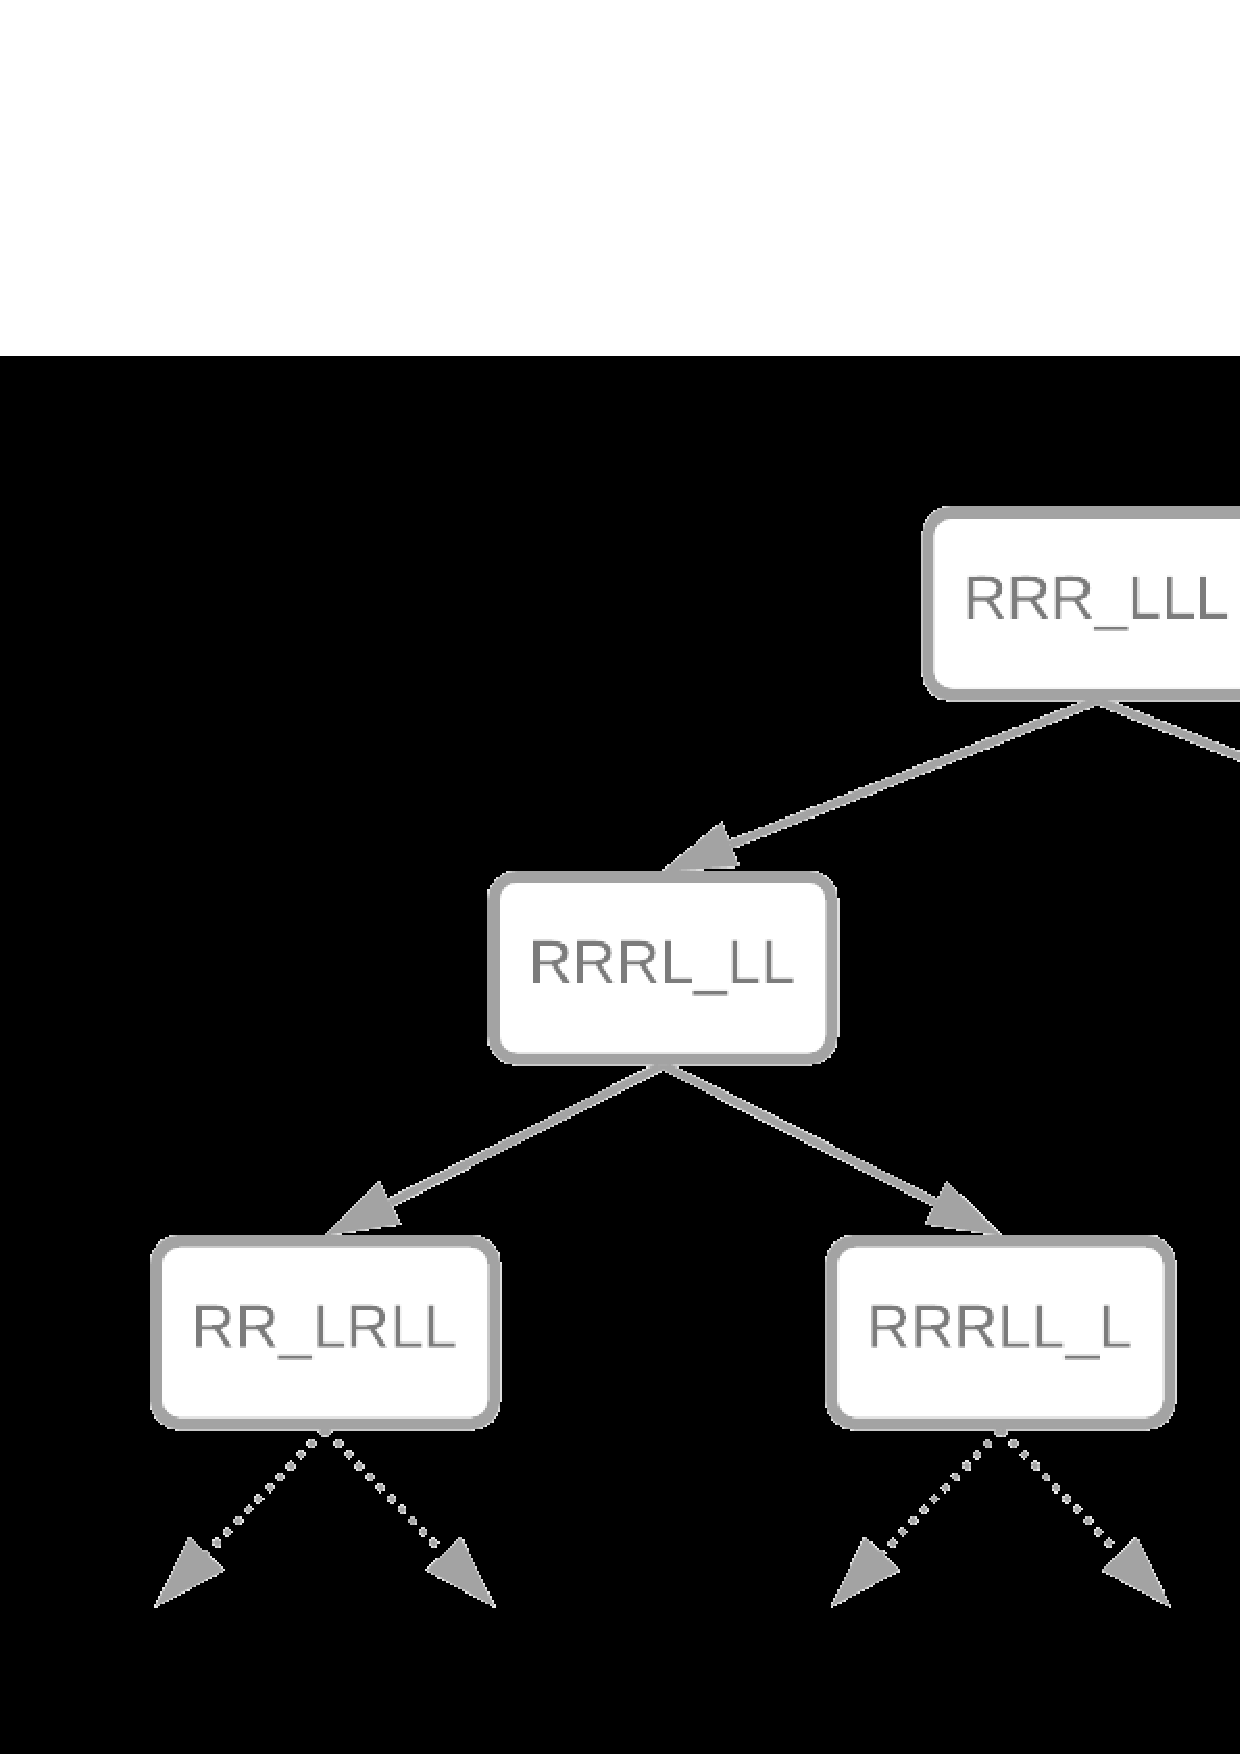
\includegraphics[width=2.5in]{rabbitleap.png}
\caption{State Space of the Rabbit Leap problem}
\label{fig_sim}
\end{figure}

Thus, the Rabbit Leap problem is just an instance of the state space search. The state space along with the moves can be thought of as a graph,
where each edge is a move.

\subsection{Size of the state space search}

The state space of the Rabbit Leap problem, contains all the states reachable by start state, using some number of moves.
One important thing to note is that, for any two states $u$ and $v$, there is at most one directed path that connects $u$ and $v$.
This is because, the movement of the rabbits can only be in one direction (left for left-bound rabbits and right for right-bound rabbits).
Thus, the state space graph is a tree (acyclic connected graph).

Now, since the $7$ letters used in the string to represent a state can vary by a total of $\frac{7!}{3!3!} = 140$, the upper bound on the size of the state space is thus $140$.
Note the actual number of states the search algorithms described later, are going to explore might be much less than $140$.

\subsection{Breadth First Search Solution}

The Breadth first search solution, first explores all the states that are at the same depth in the state space tree,
and then explores all the states of the next depth and so on.
Here is an algorithm that represents the Depth First Solution to this problem.

\begin{algorithm}
\caption{Breadth First Search}\label{BFSrabbit}
\begin{algorithmic}[1]
\Procedure{BFS}{$s,g, start$}\Comment{the state graph, the goal and start state}
\State $visited \gets \{\}$
\State $frontier \gets \{start\}$ \Comment{frontier is a queue.}
\While{$frontier.size$ $\neq$ 0}
\State $curr \gets frontier.dequeue()$
\If{$curr = gl$}
\State \textbf{return} $start \rightarrow curr$
\EndIf
\State $frontier.enqueue(curr.children \notin visited)$
\State $visited \gets visited + \{curr\}$
\EndWhile\label{bfsendwhile}
\EndProcedure
\end{algorithmic}
\end{algorithm}

Now, since BFS first visits all the states at depth, say $d$, in the state tree, whenever it gets a solution
we can say that this solution is $d$ moves away from the starting state and that no other solution exist with less than $d$
moves (because then BFS would get the solution at less than $d$ depth only). \textbf{So, the solution obtained by BFS is the optimal one}.

\subsection{Depth First Search Solution}

The DFS solution, first explores all the nodes of a branch with increasing depths, and then backtrack to choose a different
branch to explore. The algorithm of Depth First Search is given below.

\begin{algorithm}
\caption{Depth First Search}\label{BFSrabbit}
\begin{algorithmic}[1]
\Procedure{DFS}{$s,g, start$}\Comment{the state graph, the goal and start state}
\State $visited \gets \{\}$
\State $frontier \gets \{start\}$ \Comment{frontier is a stack.}
\While{$frontier.size$ $\neq$ 0}
\State $curr \gets frontier.pop()$
\If{$curr = gl$}
\State \textbf{return} $start \rightarrow curr$
\EndIf
\State $frontier.push(curr.children \notin visited)$
\State $visited \gets visited + \{curr\}$
\EndWhile\label{bfsendwhile}
\EndProcedure
\end{algorithmic}
\end{algorithm}

As it is evident from the algorithm above, there is very little difference between DFS and BFS solutions. In BFS we have
chosen a queue to store the frontier states, while in DFS a stack is used. Thus, in stack whenever a node is added it is going
to be explored immediately. This enforces the Depth First Search.

\section{Challenge Problem: Jigsaw Puzzle}
\subsection{Introduction}

The problem is pretty clear. We have to design an intelligent agent to solve a jigsaw puzzle. The first assumption we are taking is, that
every input image will have a resolution of $512 \times 512$. The second assumption, is that the total number of blocks in the jigsaw is
exactly $9$ and each block is a square. We will take an image, initially unscrambled, scramble it and then try to solve it with our agent.
The programming language we are going to use is MATLAB\textsuperscript{$\copyright$}.

\subsection{Discussion of solution}

The problem is not straightforward to solve. In this problem, the goal state is not defined (we can identify the goal state, but the
computers cannot). Hence this problem is a classic example of Simulated Annealing. In Simulated Annealing, we define the entropy of each
state and the objective is to minimize the entropy using probabilistic jumps. Assume that this entropy of any state $s$ is defined as:
\[
    E(s), \text{ where} \min{(E(s))} = E(goal)
\]

At any moment of time, simulated annealing picks up any two blocks of the image. Assume that the initial state is $i$ and the state
obtained after swapping these two blocks is $f$. Then simulated annealing does the following:

\[
     \begin{cases}
       \text{swap,} &\quad\text{if } E(f) < E(i)\\
       \text{swap,} &\quad\text{with a probability of } e^{\frac{E(i) - E(f)}{c}} \text{ if } E(f) > E(i)\\
       \text{do nothing,} &\quad\text{otherwise}\\
     \end{cases}
\]

Now, solving this problem depends on whether there is such Entropy function or not. This is exlored in the next section.

\subsection{The Entropy function}

As soon as we scramble an image, we are disturbing the smoothness of that image. This roughness occurs at the common edges of the square
blocks. The more the square blocks are not in their position, the more the roughness is going to be. The way to measure this roughness,
mathematically, is to find out how sudden is the change in the values of the pixels occuring. The gradient of a function exactly represents this
quantity.

To verify whether this works or not, we tried different gradient plots for different scrambled states of the images, and the table \ref{tab:grad}
shows the total gradient of different states compared to the total gradient of the original state.

\begin{table}[!h]
\renewcommand{\arraystretch}{1.3}
\caption{Gradient Variations}
\label{tab:grad}
\centering
\begin{tabular}{c||c||c}
\hline
\bfseries No of blocks out of position & \bfseries Total Gradient & \bfseries \% increase\\
\hline\hline
0 & 1824165.5 & 0.00\\
3 & 1840341.5 & 0.89\\
6 & 1876673.5 & 2.88\\
7 & 1885794.0 & 3.38\\
10 & 1.9294755 & 5.77\\
\hline
\end{tabular}
\end{table}

The surface plots of the gradients of original image and a scrambled image is given in figure \ref{img:scr}.

\begin{figure}[!h]
\label{img:scr}
\minipage{0.5\linewidth}
  \includegraphics[width=\linewidth]{less_scrambled_gradient.pdf}
  \caption{Original Image}
\endminipage\hfill
\minipage{0.5\linewidth}
  \includegraphics[width=\linewidth]{scrambled_gradient.pdf}
  \caption{Scrambled Image}
\endminipage
\end{figure}

It is evident from the picture that the scrambled image has a higher gradient than the original image.
So, we can say that the roughness increases as the number of blocks out of position in the image increases.

Thus, after a lot of exploration, we can say that the absolute sum of gradients of the pixel array of any image can act
as the Entropy for Simulated Annealing. The entropy function can be written as in equation \ref{eq:entr}.
\begin{equation}
E(I(x,y)) = \sum_{x,y} |\nabla I(x,y)|
\label{eq:entr}
\end{equation}

\subsection{Implementation}

The implementation of the simulated annealing is given in Algorithm \ref{algo:sim}. The matlab live code file can be found at the link
provided above.

\begin{algorithm}
\caption{Simulated Annealing}\label{algo:sim}
\begin{algorithmic}[1]
\Procedure{Simulated Annealing}{$img$}\Comment{img is the $2-$D array of pixels of the image.}
\State $iterations \gets 100$
\State $it \gets 0$
\State $i \gets img$ \Comment{Start state is the original image.}
\State $C \gets 1000$
\While{$it \neq iterations$}
\State $f \gets $ rand\_swap\_block() \Comment{random swapping}
\If{$E(f) \leq E(i)$}
\State $i \gets f$
\ElsIf{$rand(0, 1) \leq e^{\frac{(E(i) - E(f))}{C}}$}
\State $i \gets f$
\EndIf
\State $it \gets it + 1$
\EndWhile
\State \textbf{return } $i$
\EndProcedure
\end{algorithmic}
\end{algorithm}

\end{document}
